

\section{Results and Discussion}
The analysis and calculations were conducted using the R programming language \cite{R} and Python Jupyter Notebooks \cite{IPython:2007}. The scripts are included in the appendix of this report. \ref{r_scripts} All uncertainties stated are provided for a 95 \% confidence interval. The uncertainties were modelled with the aid of \texttt{METAS UncLib}, a Python uncertainty modelling library by the Swiss institute of metrology METAS.\cite{unclib}


\subsection{Conductivity of differently treated water samples}

For the different types of water specific conductivities were found to be:

\begin{table}[H]
\centering
\begin{tabular}{
    l
    l
}
\hline
water treatment & $\kappa$ / \textmu S/cm \\ \hline
tap             & 283(14)  \\
deionized       & 2.85(12) \\
degased         & 1.1(3)   \\ \hline
\end{tabular}
\caption{Specific conductivities $\kappa$ of differently treated water samples.}
\end{table}

The measured specific conductivity for the purified, degassed water exceeds the manufacturer specifications of \qty{0.055}{\micro\spc} by a substantial amount.\cite{huber} To accurately measure such low conductivities, a closed measurement apparatus, where no oxygen is absorbed, would be required.



\subsection{Correlation between temperature and conductivity}

The thermal coefficient of the potassium carbonate conductivity was found to be $\alpha_{\mathrm{K_2CO_3}} =$ \qty[per-mode=reciprocal]{0.02143 \pm 0.00008}{\per\kelvin}, and thus closely matching the approximately \qty[per-mode=reciprocal]{0.02}{\per\kelvin} typical for aqueous solutions.\cite{meister} The conductivity at standard conditions was determined at $\kappa(\qty{25}{\celsius}) =$ \qty{19.58 \pm 0.06}{\milli\spc}.

\begin{figure}[H]
    \centering
    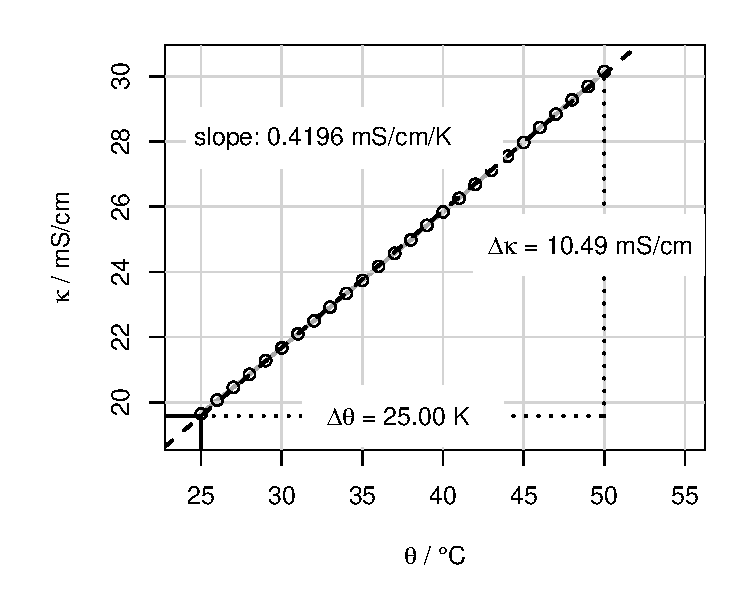
\includegraphics[width=.45\textwidth]{figures/plots/lfk_temperature.pdf}
    \caption{The specific conductivity of potassium carbonate as a function of the temperature of the solution. The correlation is perfectly linear ($\mathrm{R}^2 > 0.9999$).}
    \label{fig:lfk_temp}
\end{figure}



\subsection{Molar conductivity of sodium carbonate and potassium carbonate}

From three conductivity measurements of \qty{0.01}{\M} $\mathrm{K_2CO_3}$ and $\mathrm{Na_2CO_3}$ each, molar conductivities of $\Lambda_{\mathrm{K_2CO_3}} = $ \qty{216 \pm 4}{\Smolar} and $\Lambda_{\mathrm{Na_2CO_3}} = $ \qty{131.1 \pm 0.6}{\Smolar} respectively were determined.


\subsection{Limiting molar conductivity of potassium carbonate}

By recording conductivities at varying concentrations of $\mathrm{Na_2CO_3}$, the molar conductivity extrapolation to $c = $ \qty{0}{\M} returns $\Lambda^0_{\mathrm{Na_2CO_3}} = $ \qty{251 \pm 7}{\Smolar}.

Using the same regression model to predict a molar conductivity for \qty{0.01}{\M} $\mathrm{Na_2CO_3}$ yields $\Lambda_{\mathrm{Na_2CO_3}} = $ \qty{142 \pm 9}{\Smolar}, thus confirming the above recordings with just a slight variation, which is probably due to the differences in the experimental setup.

\begin{figure}[H]
    \centering
    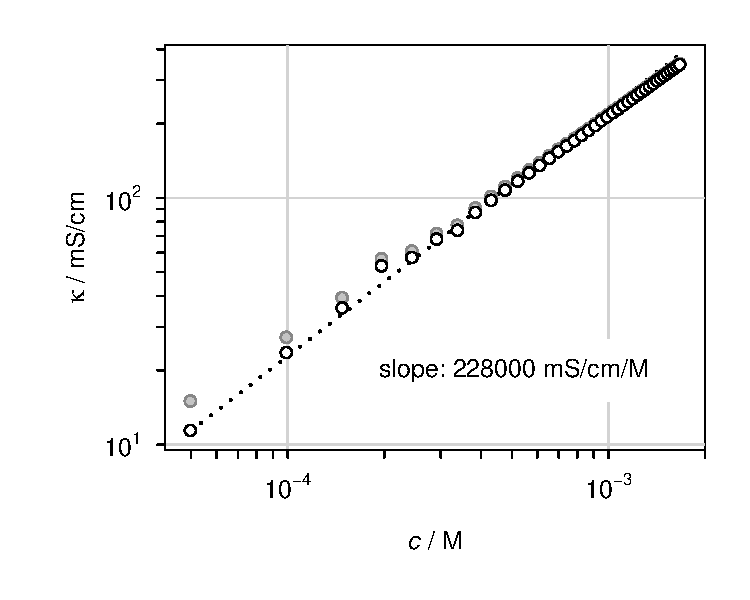
\includegraphics[width=.5\textwidth]{figures/plots/lfk_molar_1.pdf}
    \caption{Plotting the specific conductivity $\kappa$ against the concentration $c$ confirms the proportional relationship (dotted line), and thus legitimizes the consistency of the molar conductivity across the entire range of dilution. \\ The grey points show the raw conductivity recordings, the white points are corrected for the conductivity of the pure water. For further processing, the corrected values were used.}
    \label{fig:lfk_molar_1}
\end{figure}

\begin{figure}[H]
    \centering
    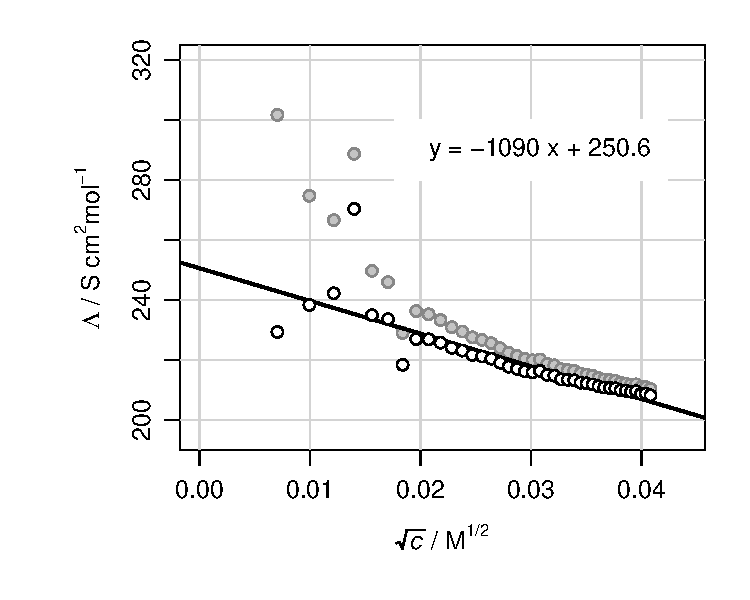
\includegraphics[width=.5\textwidth]{figures/plots/lfk_molar_2.pdf}
    \caption{Extrapolation to the limiting molar conductivity in accordance with \textit{Kohlrausch's square root law}. (Eq. \ref{eq:kohlrausch})}
    \label{fig:lfk_molar_2}
\end{figure}


\subsection{Conductometric titration}

\begin{figure}[H]
    \centering
    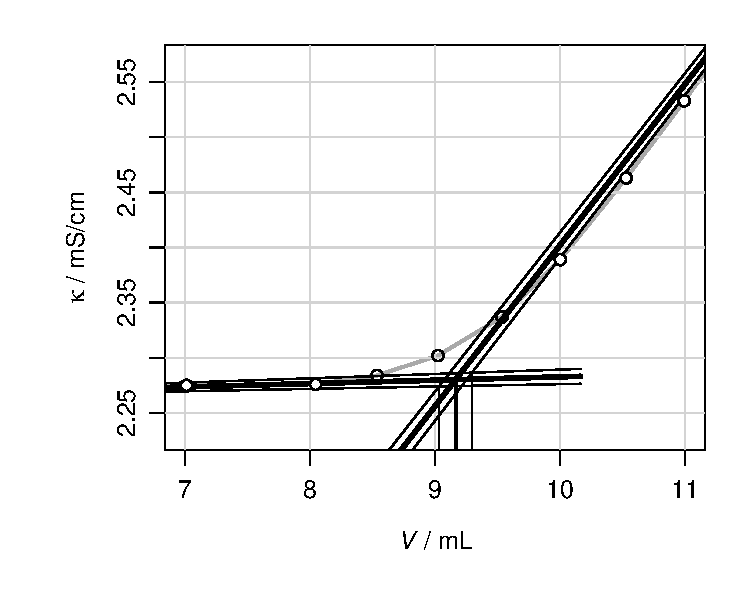
\includegraphics[width=.5\textwidth]{figures/plots/lfk_titration_zoom.pdf}
    \caption{Magnified view of the equivalence point in the titration of $\mathrm{K_2CO_3}$ with \qty[round-precision=5]{0.09997}{\M} $\mathrm{CaCl_2}$. The transparent points were not included in the calculation of the intersection point. The full titration plot can be seen in the appendix.\ref{fig:lfk_titr_full}}
    \label{fig:lfk_titr_zoom}
\end{figure}

\columnbreak

Intersecting the lines before and after the equivalence points of the conductometric titration (where $\kappa_1(V_{\mathrm{pre}}) = \kappa_{\mathrm{post}}(V_t)$) yields a titer volume $V_t =$ \qty{9.2 \pm 0.3}{\milli\litre}, which corresponds to an initial concentration of \qty{9.2 \pm 0.3}{\milli\M} of the $\mathrm{K_2CO_3}$ solution. The uncertainty interval was derived with the formula
\begin{equation}
    c_{\mathrm{\overline V_t}} = 2 * 
    \frac{s_{\mathrm{\overline V_t,post}} + s_{\mathrm{\overline V_t,pre}}}{a_{\mathrm{\kappa,post}} - a_{\mathrm{\kappa,pre}}}
\end{equation}

\iffalse{


%hi wie gehts voran? :)
%sameeeeeeee ich muss noch die leitfähigkeitstitration schrieben, dann bin ich fertig mit experimental, bis auf die chemikalien, da könnte ich eventuell kurz deine hilfe benötigen ( : 0 heiligenschein emojiiiiii) ah so geht das hahahha wenn man das verkehrt herum anscaut ist es ein orang utan mit offenem mund hahaha HAHAHAHAHAHAHAH
% :party-emoji:
% salut, ça va ?
% jetzt komm ich langsam in den Flow :)
% 

%
% (==)
% .  .
% -__-
% hahahah HA hahahhahah na gut, aber dann schau ich mal, dass ich das schnell fertig bekommen hihi und dann schau ich nochmal vorbei
% well das sieht eher aus wie ne creepy Katze... (holy cat!)
% ich hoffe auch dass ich das Zeugs in 1h fertig kriege. Dann kann ich gerne bei dir mithelfen :)
% :)))))))) dankööö boah diese reports kacken mich so an, unfassbar haha, so unnnnnnnötig, weil wir nix spannendes gemacht haben :*( so wenns wenigstens eine synthese gewesen wäreeeeeeee

% honestly bin ich froh um die Abwechslung vom AC Lab hahaa. Dort sind die Auswertung sooooo ööööde. Hier lerne ich irgendwie mehr finde ich.
%ok, das stimmt auch widerum haha
%\newpage
%hi hihihihihi weißt du zufälligerweise noch, welche chemicals wir in welchem experiment verwendet haben? 
% hmmmmmmm hahaha cry crycrycrycrycry . lemme see... dontcryeverythingwillbeok :) :))
% fotografiert habe ich: sodium carbonate, potassium carbonate, die fotos hast du mir schon geschickt :))
%im buch ist nämlich der graph mit sodium chloride und calcium chloride
% wollen wir mal im chat fragen?
%guter plan 
%soll ich machen?
% ooOOOOHHHH WAIT, MAN MUSS JA NUR INS LAB JOURNAL SCHAUN! :D XD
% Temperaturabhängigkeit: K2CO3hä wie hast du das jetzt da rausgelesen lol hahahahahaha
% weil ich aufgeschrieben hab dass ich 138.91 g K2CO3 eingewogen hab :)
% UUUUUUNNNNDDD molar conductivity steht m(Na2CO3) = 0.5298 g
% uuuuuunnnnd bei der Titration hatten wir ja die vorgefertigte Lösung K2CO3

%ich hab im excel stehen, dass wir molar mit beiden gemacht haben und konzentrationsabhängigkeit nur mit natrium

% ahjaaaa omg Janosch kann einfach nicht lesen
% eine Zeile darüber ssteht noch K2CO3 :see-no-more-monkey:cryyyyyyyyyyyyyyyyyyyyyyyyy omg wie wisssen wir einfach gar nix mehr von dem lab....? bei ddr wusste ich noch alles :(
% jaaa aber es war auch fürchterlich stressig und nichts wurde kommuniziert von den Assistenten. Ich mag mich nicht mal mehr erinnern bei wem wir das Experiment gemacht hatten, hätte die nicht eine E-Mail geschrieben hahahaha
%hahahhahaha
%aber was ist jetzt mit kso3?? hooppla C statt S. =>K2CO3 <=
% mannomann ich brauch eiine Pause... geh jeztt was essen.
%tu das ahahhaha ich glaub wir haben einmal abgewogen und dann einfach mit wasser aufgefüllt fürs nächsste experiment, damit die konzentration sich verändert... aber bin mir nicht mehr sicher welche chemikalie wann das erste mal verwendet wurde.... haben wir einen vorlage bericht für lfk?? OMG ICH WEISS ES WIEDER

\subsection{Density and refractive index}

The refractive index and density of acetone were measured at 

$n_D^{20} =$ \qty{1.35867}{1} and 

$\rho = $ \qty{0.7913}{\density} (\textit{method B}) 
\\and the density of acetone was calculated (\textit{method A}) to be 

\qty{0.7904 \pm 0.0026}{\density} 
\\corresponding with literature values of 

$n_D^{20} =$ \qty{1.3588}{1} and 

$\rho = $ \qty{0.7899}{\density}. \cite{meister} 
\\For n-hexane values of 

$n_D^{20} =$ \qty{1.37506}{1} and 

$\rho = $ \qty{0.6594}{\density} (\textit{method B}) and 

$\rho = $ \qty{0.6572 \pm 0.0022}{\density} (\textit{method A}) 
\\were obtained compared to literature values of 

$n_D^{20} =$ \qty{1.3751}{1} and 

$\rho = $ \qty{0.6603}{\density}. \cite{meister} 
\\It can be observed, that the results obtained for acetone are more precise than those of n-hexane. This could be explained for example by the varying grades of purity (99.5\% vs. 95\% specified by their producers.
\begin{figure}[H]
    \centering
    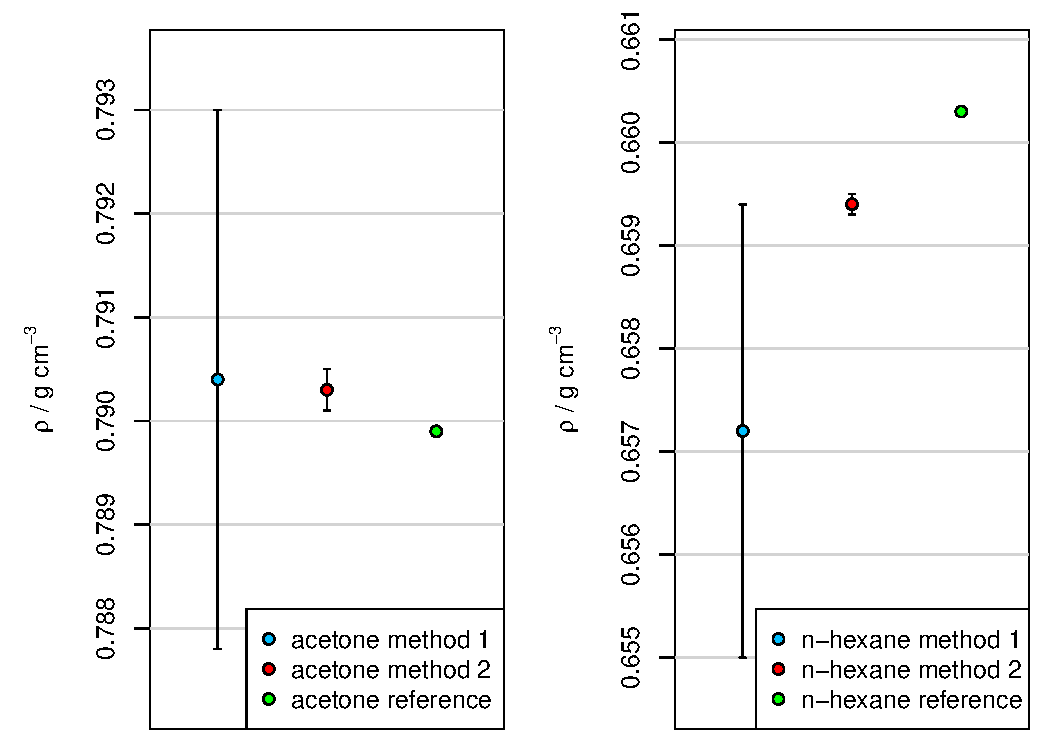
\includegraphics[width=.5\textwidth]{figures/rho-comparison.pdf}
    \caption{Comparisons of the density values measured, and reference values found in literature \cite{meister}.}
    \label{fig:rho_comp}
\end{figure}


\subsection{Vapor Pressure}

\begin{figure}[H]
    \centering
    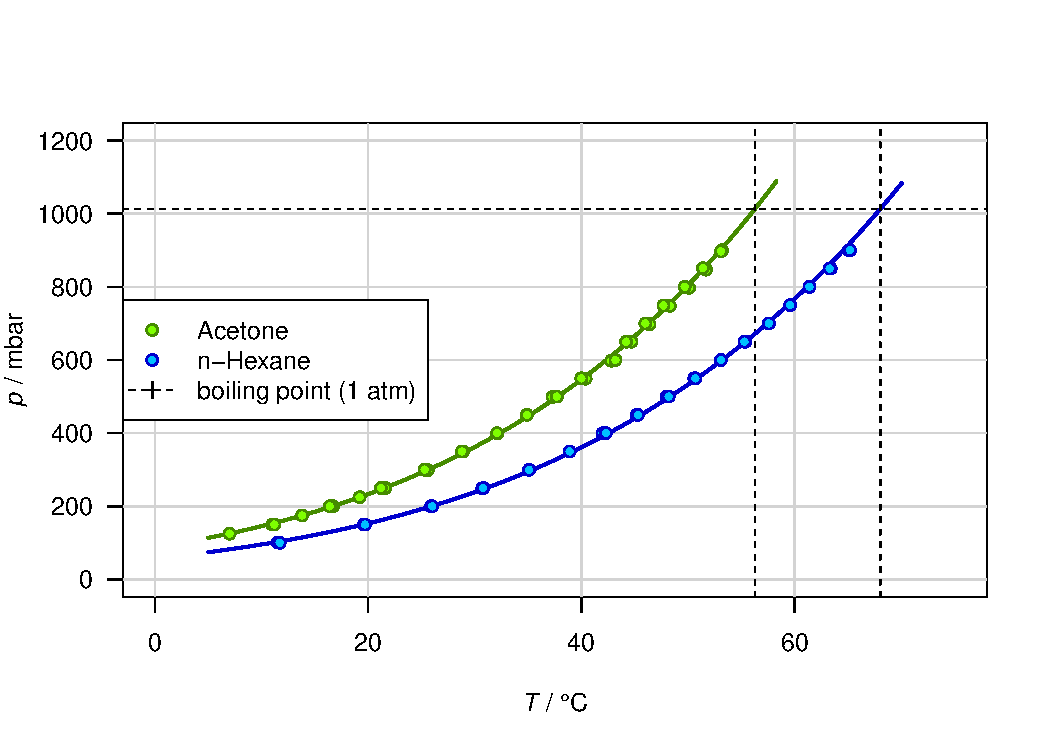
\includegraphics[width=.5\textwidth]{figures/DDR1_t_p.pdf}
    \caption{The vapor pressure curves illustrate the exponential correlation between vapor pressure and temperature. (Standard boiling points extrapolated and marked by the vertical and horizontal lines.)}
    \label{fig:ddr1_t_p}
\end{figure}

As mentioned in the introduction, vapor pressure can be described as $p(T)$. Accordingly, the results obtained from measuring the samples' boiling temperatures at differing surrounding pressures were plotted in a $p$-$T$-diagram, presented in Fig. \ref{fig:ddr1_t_p}.

Enthalpies of vaporization were calculated with by plotting logarithmic $\frac{p}{p_0}$ against inverse temperature $T$ via a linear regression model (Fig. \ref{fig:ddr1_inv_ln}) and calculating the slope $b$ of the resulting linear graphs. Expansion of equation (\ref{eq:6.2}) shows that it is equal to $\frac{\Delta_VH}{R}$. Results amounted to 

$\Delta_VH=$ \qty{32.49 \pm 0.26}{\kJpmole} for acetone and 

$\Delta_VH=$ \qty{32.66 \pm 0.25}{\kJpmole} for n-hexane. 
\\Acetone is a polar solvent and n-hexane is not. Because of this, one would assume, that its enthalpy of vaporization and standard boiling temperature would be higher than those of n-hexane because of stronger intermolecular bonds. Evidently, this is not the case. A possible explanation could be that though it is polar, acetone has a lower molar mass than n-hexane, meaning it would take less  energy to bring one mol of acetone from its fluid to its gaseous form than one mol of another substance with similar polarity.

 
\begin{figure}[H]
    \centering
    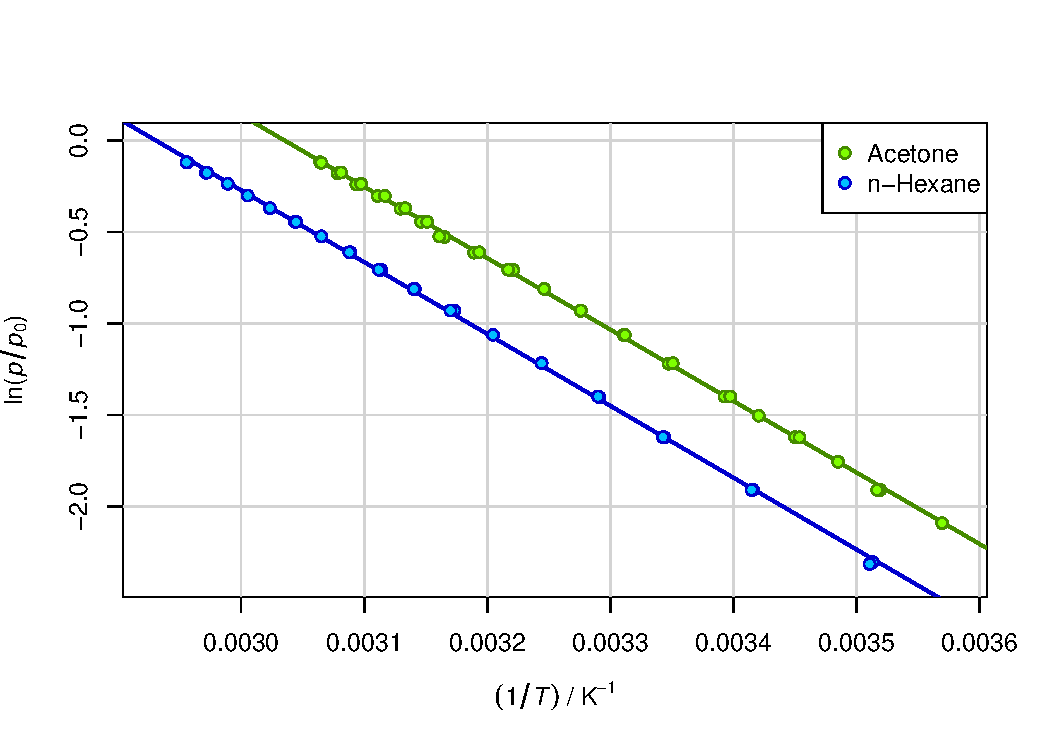
\includegraphics[width=.5\textwidth]{figures/DDR1_inv_ln.pdf}
    \caption{The Enthalpy of vaporization for each sample can be visualized in a $\ln\left(\frac{p}{p_0}\right)$ - $\frac{1}{T}$ diagram, because it is directly proportionate to the linear graph's slope $b$ (by factor of the gas constant $R$.)}
    \label{fig:ddr1_inv_ln}
\end{figure}


Normal boiling temperatures $T_0$ and standard entropies $\Delta_VS(T_0)$ of vaporization were also calculated with the help of the linear model parameters intercept $a$ and slope $b$ and found to be 

$T_0^{\text{acet}}$ = \qty{56.29}{°C}  

$T_0^{\text{nhex}}$ = \qty{68.06}{°C}
\\corresponding to literature values of 

$T_0^{\text{acet}}$ = \qty{56.15 \pm 0.3}{°C} 

$T_0^{\text{nhex}}$ = \qty{68.75 \pm 0.3}{°C}

and

$\Delta_VS(T_0)^{\text{acet}}$ = \qty{98.62}{\joule\per\mole\per\kelvin}

$\Delta_VS(T_0)^{\text{nhex}}$ = \qty{95.74}{\joule\per\mole\per\kelvin}.





\subsection{Transient evaporation cooling}
The data files generated by the \texttt{TREVAC} apparatus were imported to R. With the \mintinline{R}{identify()} command, the relevant time ranges for the peak integration could be selected graphically. (Fig. \ref{fig:nhex_peaks}) This data, including statistical parameters were then exported to a \textit{csv} file for documentation purposes and for further processing. To calculate the final values, including standard errors, a Jupyter notebook \cite{IPython:2007} with the \texttt{METAS UncLib} uncertainty modeling software \cite{unclib} was used. Formula \ref{eq:6.18} was 

For acetone, \qty{30.2 \pm 2.8}{\kJpmole} was calculated, and for n-hexane, \qty{32.0 \pm 1.9}{\kJpmole}, was found.

\begin{figure}[H]
    \centering
    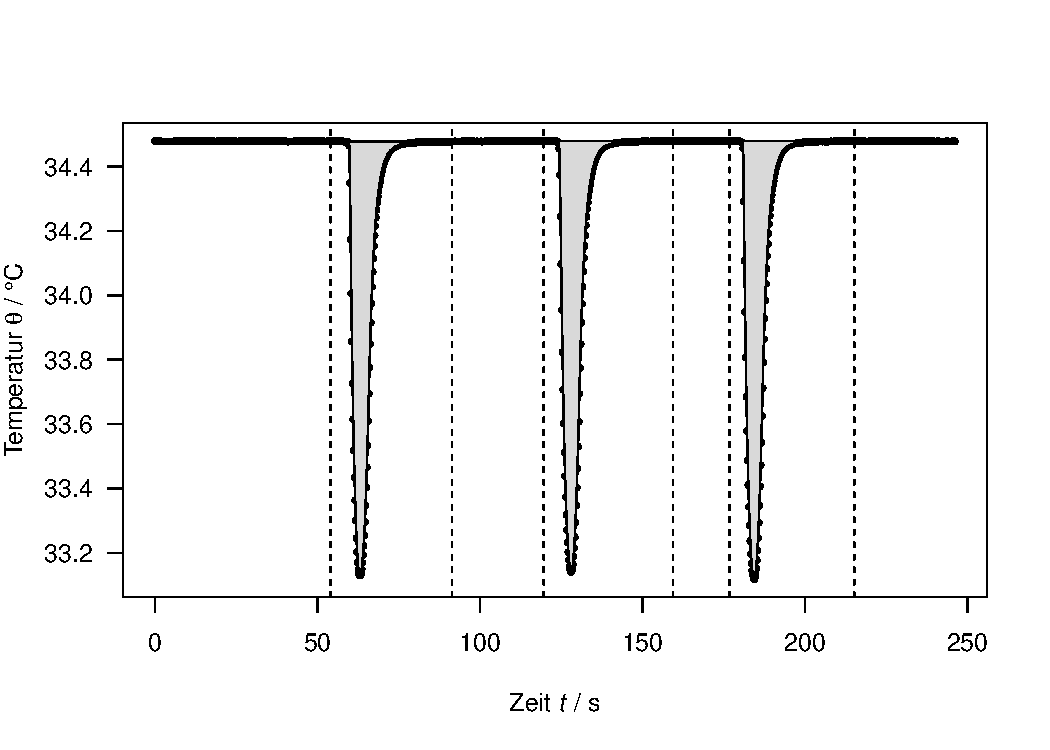
\includegraphics[width=.5\textwidth]{figures/n-hexane.pdf}
    \caption{Temperature peaks caused by n-hexane withdrawing heat from the measurement surface. The grey area is directly correlating with the enthalpy of evaporation $\Delta_VH_{\text{subst}}$ of the substance.}
    \label{fig:nhex_peaks}
\end{figure}

Standard values for $\Delta_VH$ can be found on the website of the \texttt{National Institute of Standard Technology}:

$\Delta_VH^0_{\text{acet}}$ = \qty{31.27}{\kJpmole} \cite{NIST:acet}

$\Delta_VH^0_{\text{nhex}}$ = \qty{31\pm 1}{\kJpmole} \cite{NIST:nhex}

}